Notre système, visible à la figure \ref{architecture}, s'architecture autour du \textit{message broker} Kafka \cite{kafka}. Les contrôleurs KNX et Openzwave gèrent respectivement les stores et les radiateurs ainsi que les lumières et capteurs multi-fonctions (présence, luminance, température, humidité). Ils peuvent d'une part recueillir les informations des \textit{devices} associés, mais également attribuer des nouvelles valeurs pour chacuns. Un utilisateur muni de l'application mobile et se trouvant à portée d'un Beacon peut intéragir avec les \textit{devices} de la pièce (\textit{room}) associée avec le Beacon. Ces interactions comportent la visualisation de l'état actuel des \textit{devices} (présence, niveau de température, d'humidité et de lumière, ouverture des stores et des radiateurs) mais aussi leur contrôle (lumière, stores et radiateurs). L'application échange avec un serveur HTTP \acrshort{rest} qui fait office de \textit{backend}, lisant dans la base de données les relations entre Beacons, pièces, \textit{devices} et utilisateurs. Un module d'authentification (non implémenté) vérifie qu'un utilisateur dans une pièce donnée a le droit d'utiliser les \textit{devices} associés. La base de données garde également en mémoire les données des \textit{devices}, pour des éventuelles statistiques. Un module indépendant lit la base de données pour produire dans Kafka la liste des \textit{devices}  pour les mettre à disposition des modules KNX et Openzwave. Le module "Automatic Controller" exécute des actions de manière automatique et intelligente, selon certaines conditions, par exemple si quelqu'un se trouve dans une pièce alors qu'il fait sombre, la lumière s'allume.

\begin{figure}
    \begin{center}
        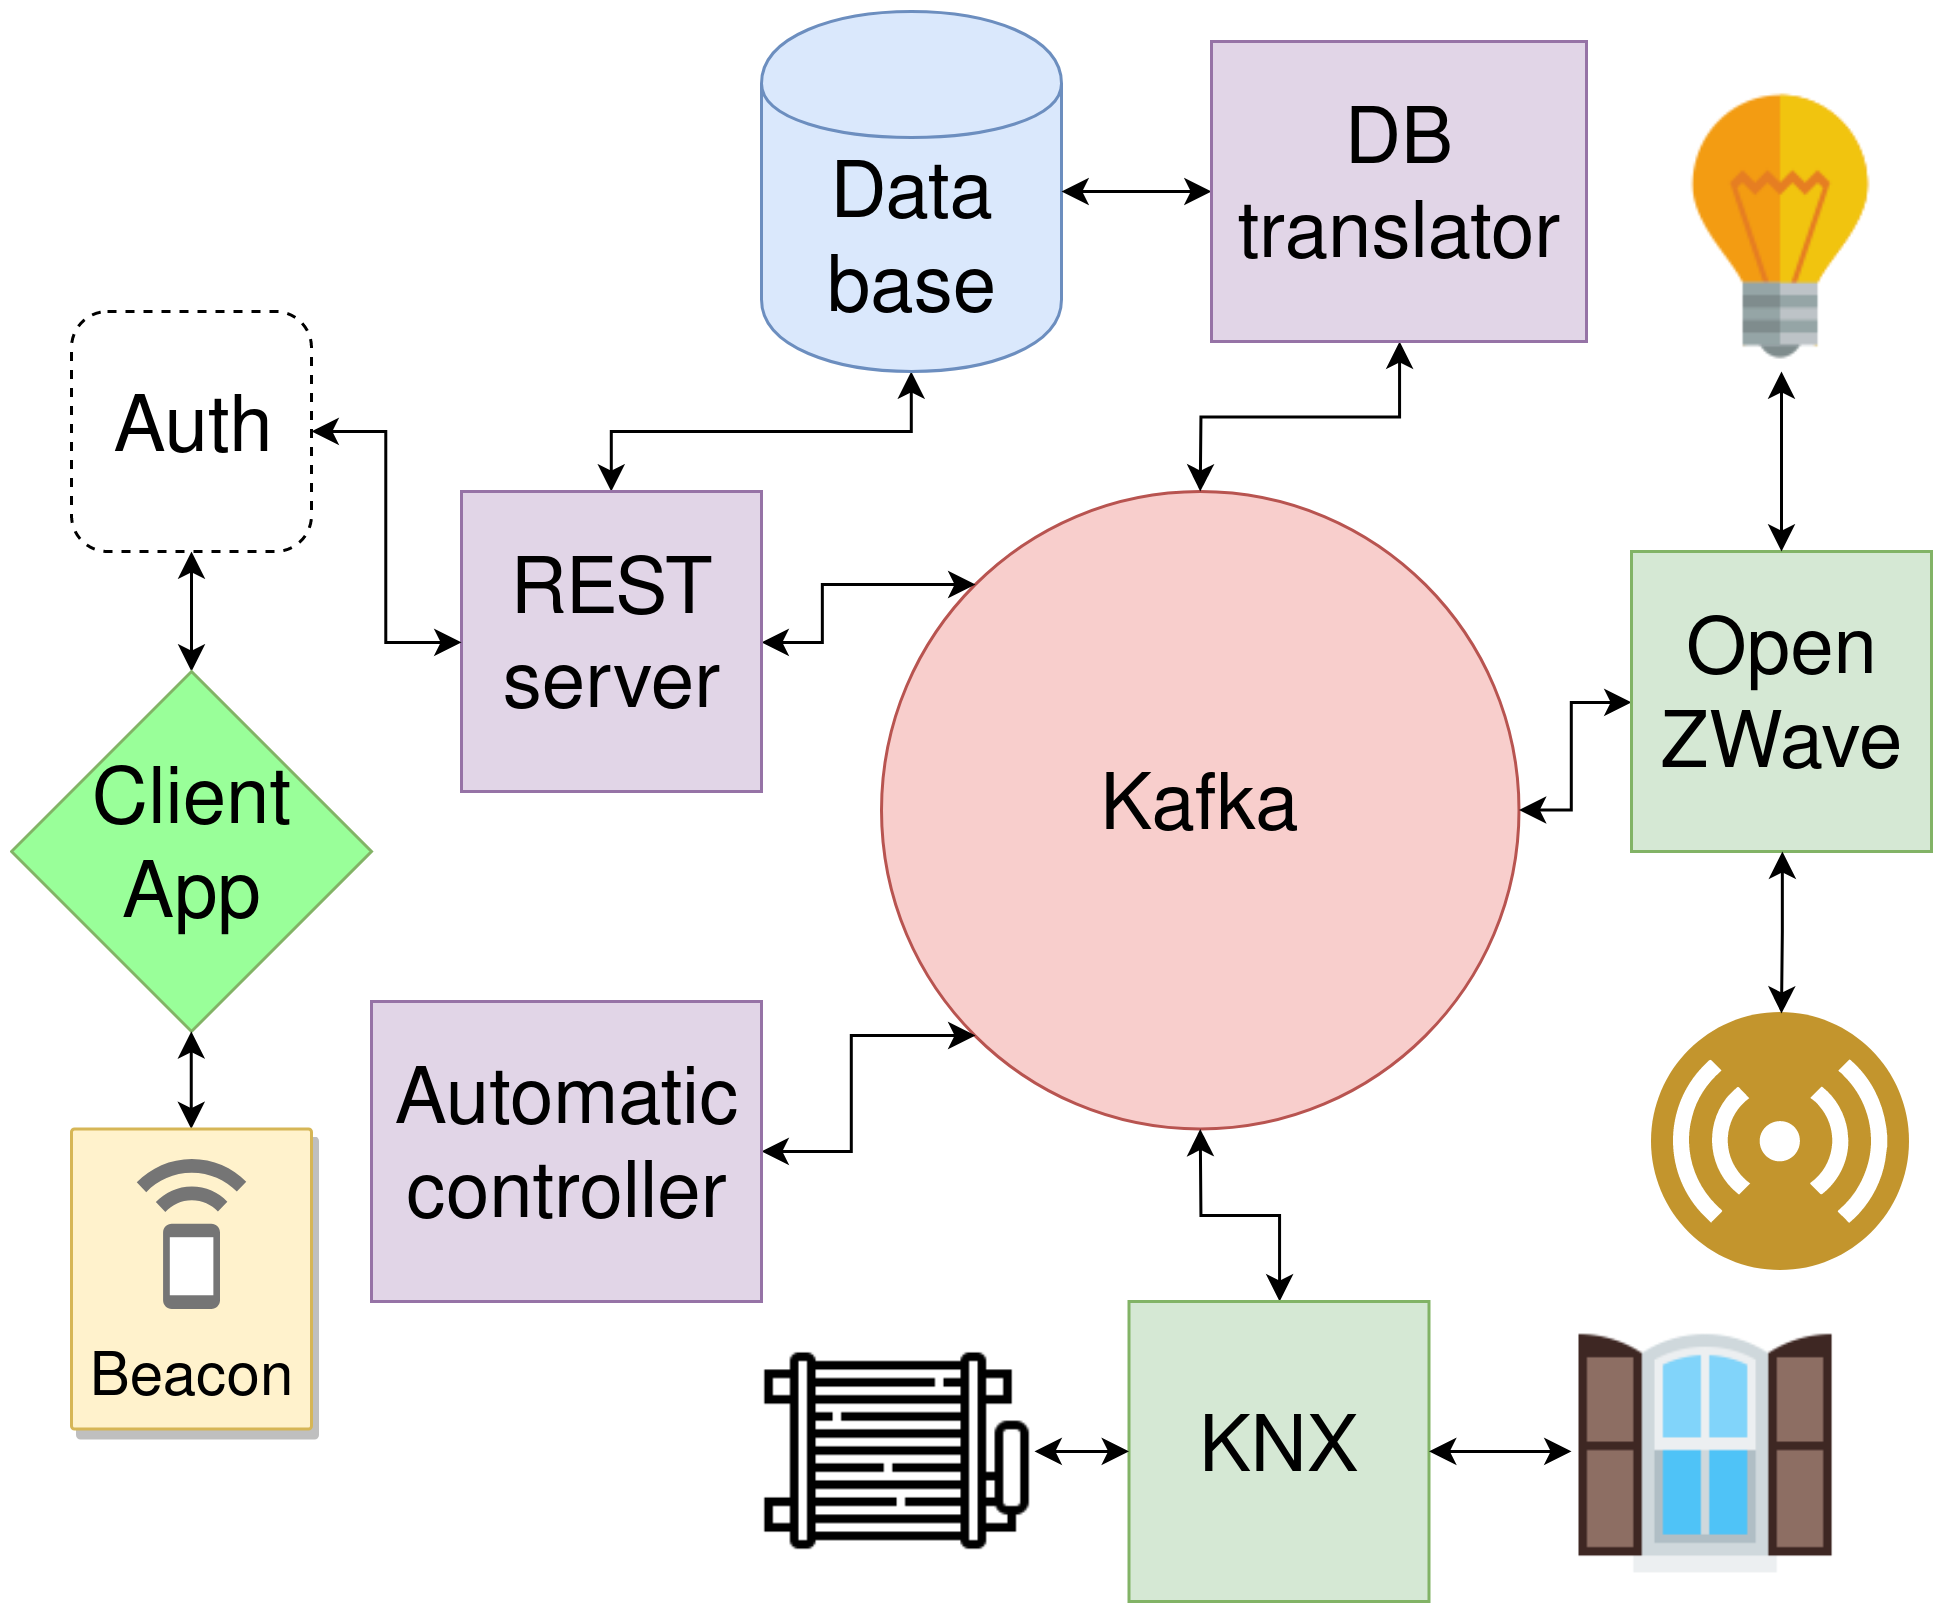
\includegraphics[width=1\textwidth]{img/architecture.png}
    \end{center}
    \caption{Architecture globale du système}
    \label{architecture}
\end{figure}
